\section*{Motorik und Sensorik}

\paragraph{Übersicht Motorik}
\begin{itemize}
  \item Motorik = Gesamtheit der Aktionen der Muskulatur
  \item \textbf{Sensomotorik}: Zusammenhang zwischen Sinneseindrücken und Muskelaktivität (Steuerungs- und Regelsysteme)
  \item \textbf{Psychomotorik}: Zusammenhang zwischen geistig-seelischer Verfassung und Körperbefindlichkeiten (Gestik, Körperhaltung,\dots)
\end{itemize}

\paragraph{Übersicht Sensorik}
\begin{itemize}
  \item Sensorik (in Technik) = Sensoren nutzen für Messung + Regulation von biologischen/technischen Systemen
  \item Üblicherweise: Verwendung von \emph{Einheitssignalen}
\end{itemize}

\paragraph{Muskulatur --- Struktur}
\begin{itemize}
  \item Motorische Endplatte: überträgt elektrischen Nervenfaser-Reiz als chemischen Impuls an Muskelfaser (chemische Synapse, Neurotransmitter Acetylcholin)
  \item Muskel \( \to \) Muskelfaser-Bündel \( \to \) Muskelfaser \( \to \) Muskelfibrille \( \to \) Sarkomer \( \to \) Myosin- und Aktin-Filamente
\end{itemize}

\paragraph{Muskulatur --- zelluläre Grundlagen}
\begin{enumerate}
  \item ATP-beladene Myosinköpfchen über Troponin an Aktinfilament angedockt
  \item ATP zerfällt zu ADP und P, Ca wird abgestoßen, ADP bleibt in Myosinköpfchen
  \item Myosinköpfchen schlagen um \( \to \) Kontraktion
  \item ADP wird abgegeben, Myosinköpfchen in Endstellung
  \item Aktin-Myosinbindung wird gelöst, Myosinköpfchen durch ATP neu gespannt \\* \( \to \) ATP macht Myosinköpfchen ``weich''
\end{enumerate}

\paragraph{Muskulatur --- Kontraktion}
\begin{itemize}
  \item[=] Aktinfilamente bewegen sich zu Zentrum von dickstem Filament
  \item Bewegung durch Klappbewegung Myosinköpfchen \( \to \) Ruderbewegung
  \item ATP zur Lösung von Myosin und Aktin benötigt \( \leadsto \) Totenstarre wenn keine
\end{itemize}

\paragraph{Troponin}
\begin{itemize}
  \item[=] An Muskelkontraktion beteiligtes Strukturprotein
  \item Tropomyosinfaden blockiert Myosinbindungsstelle
  \item Muskelkontraktion \( \to \) Anstieg \( \text{Ca}^{2+} \)-Konzentration \( \to \) Bindung \( \text{Ca}^{2+} \) an Troponin \( \to \) Troponinmoleküle bewegen Tropomyosinfaden \( \to \) Kontaktstelle zwischen Aktin und Myosinköpfchen frei 
\end{itemize}

\paragraph{Motorcortex}
\begin{itemize}
  \item[=] abgrenzbarer Großhirnrinde-Bereich und funktionelles System
  \item steuert willkürliche Bewegungen
  \item Zusammenstellung komplexer Bewegungsabfolgen aus einfachen Mustern
  \item Reizleitung Motorkortex \( \to \) Rückenmark \( \to \) Nerv (siehe motorische Endplatte)
  \item \textbf{Primär-Motorische Rinde} (M1): unmittelbare Bewegungssteuerung (liegt überwiegend auf \emph{gyrus praecentralis})
  \item \textbf{Supplementär-Motorische Rinde} (SMA): Erstellen Bewegungsabfolgen aus Bewegungs-Fundus + Vorbereitung willkürlicher (bewusst + unbewusst) Bewegungen
\end{itemize}

\paragraph{Somatosensorischer Cortex}
\begin{itemize}
  \item[=] abgrenzbarer Großhirnrinde-Bereich
  \item zentrale Verarbeitung haptischer Wahrnehmungen (Tasten + Temperatur)
  \item \textbf{Mechanorezeptoren}: Sinneszellen, die mech. Kräfte in Signale wandeln
  \item Berührungs- und Druckrezeptoren:
  \begin{itemize}
    \item Vater-Pacini-Körperchen: Mechanorezeptoren auf Haut, besonders gut bei Vibrationsempfindungen
    \item Merkelsche Scheiben: Mechanorezeptoren auf Haut, Druckrezeptoren
    \item Haarfollikelrezeptoren, \dots
  \end{itemize}
  \item Wärmerezeptoren:
  \begin{itemize}
    \item Krausesche Endkolben: Ermitteln Temperatur auf Hauptoberfläche
  \end{itemize}
\end{itemize}

\paragraph{Somatotopie}
\begin{itemize}
  \item[=] Abbildung Körperregionen/-strukturen auf Nervenzellenareale im Gehirn
  \item \textbf{Homunculus}: Modell neuronale Beziehung zwischen kortikalen Bereichen und Skelettmuskeln/sensorischen Feldern \\* \( \to \) Benachbarte Körperregionen auf benachbarte Kortexgebiete abgebildet
  \item Unterscheidung sensorischer und motorischer Cortex
\end{itemize}
\begin{figure}[H]
  \centering
  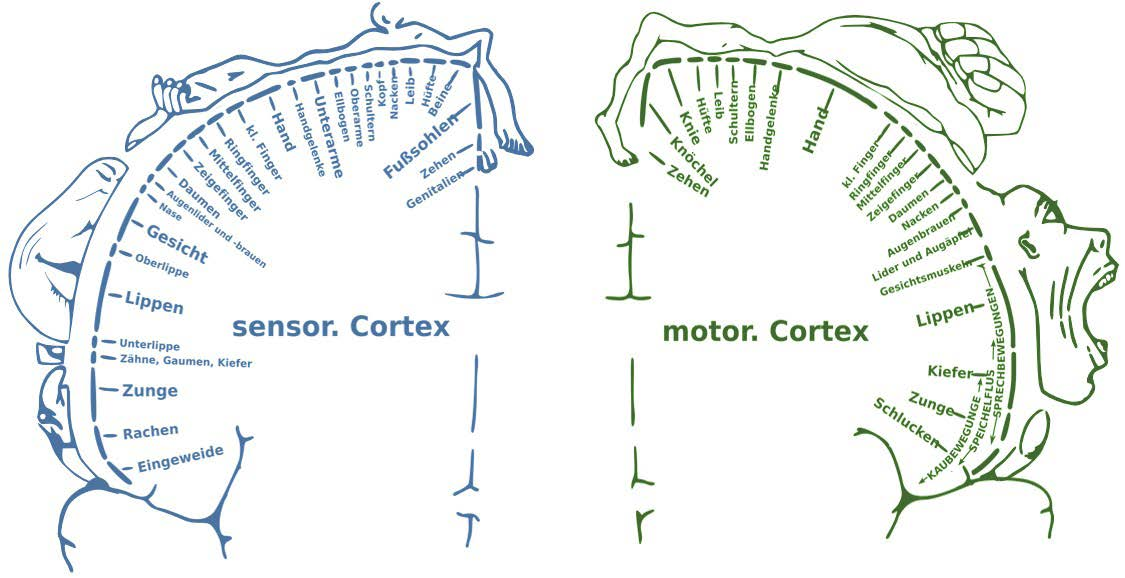
\includegraphics[width=.7\linewidth]{assets/img/homunculus.png}
\end{figure}

\paragraph{Nervenzelle --- Aufbau}
\begin{itemize}
  \item \textbf{Soma}: Zellkörper, enthält Zellkern + verschiedene Organellen (raues/glattes ER, Mitochondrien,\dots)
  \item \textbf{Dendriten}: Von Soma auswachsende, fein verästelte Zellfortsätze \\* \( \to \) Kontaktstellen für andere Zellen, Erregungsübertragung über Synapse
  \item \textbf{Axon}: Zellfortsätze, entspringen Axonhügel, Weiterleitung Erregung an andere Zellen
  \item \textbf{Synaptischer Spalt}: Zwischenraum zwischen präsynaptischer Membranregion (Präsynapse) und postsynaptischer/subsynaptischer Membranregion (Postsynapse) bei einer nachgeschalteten Zelle
  \item \textbf{Neurotransmitter}: Botenstoffe an chemischen Synapsen für Erregungsübertragung (Transmission): Acetylcholin, Noradrenalin, Dopamin, Serotonin, \dots
  \begin{enumerate}
    \item Senderzelle schüttet bei Erregung Neurotransmitter präsynaptisch aus
    \item Neurotransmitter überbrücken synaptischen Spalt
    \item Empfängerzellen-Rezeptoren empfangen postsynaptisch Neurotransmitter
  \end{enumerate}
\end{itemize}

\paragraph{Aktionspotential, Elektro-chemische Mechanismen}
\begin{itemize}
  \item \textbf{Zellmembran}:
  \begin{itemize}
    \item Lipid-Doppelschicht, lipophile Seite innen, hydrophile Seite außen
    \item Proteine mit verschiedenen Funktionen in Lipid-Doppelschicht integriert (z.B. Ionenkanäle)
  \end{itemize}
  \item Ionenkonzentration unterschiedlich \( \to \) viele \( \text{K}^+ \), wenige \( \text{Na}^+ \) im Zellinneren
  \item Ionenpumpe hält Konzentrationsgefälle aufrecht \\* \( \to \) Energiegewinnung durch ATP-Spaltung
  \item Einige \( \text{K}^+ \)-Kanäle immer offen \( \to \) \( \text{K}^+ \)-Ionen diffundieren aus Zelle heraus
  \item Gleichzeitig wenige \( \text{Na}^+ \)-Kanäle offen \( \to \) kaum \( \text{Na}^+ \)-Ionen zum Ausgleich \\* \( \to \) Zellinneres verliert positive Ladungen, negative Spannung entsteht
  \item \textbf{Ruhepotential}: Potentialdifferenz bremst Ausstrom von \( \text{K}^+ \) \\* \( \to \) Gleichgewichtszustand zwischen nach außen gerichteter Diffusions-Tendenz und nach innen gerichteter elektrischer Anziehung der \( \text{K}^+ \)
  \item \textbf{Depolarisation}:
  \begin{itemize}
    \item Axon durch elektrischen Reiz leicht depolarisiert \( \to \) einige spannungsgesteuerte \( \text{Na}^+ \)-Poren öffnen sich
    \item Depolarisation erreicht Schwellwert \( \to \) alle \( \text{Na}^+ \)-Kanäle offen, Anzahl durchlässiger \( \text{K}^+ \)-Poren zuerst gleich \\* \( \to \) Überschuss positiver Ladung im Inneren des Axons
  \end{itemize}
  \item \textbf{Repolarisation}: \( \text{Na}^+ \)-Poren schließen nach kurzer Zeit wieder, alle noch geschlossenen \( \text{K}^+ \)-Kanäle öffnen \( \to \) schneller \( \text{K}^+ \)-Ausstrom führt zu Rückkehr des Membranpotentials zu Ruhewert
\end{itemize}

\paragraph{Nervenleitung}
\begin{enumerate}
  \item Reizung an bestimmter Stelle \( \to \) Aktionspotential \( \to \)  Angrenzung positiver und negativer Ladungen ohne trennende Membran
  \item Ausgleichsströme entstehen \( \to \) Membranpotential benachbarter Stellen wird erniedrigt \( \to \) Schwellwert wird erreicht, Aktionspotential auch bei Nachbar
  \item Signal wird weiterverbreitet
\end{enumerate}

\paragraph{Signalmodulation}
\begin{itemize}
  \item Aktionspotential hat immer selbe Amplitudenform
  \item Information codiert über Frequent + Dauer der Entstehung von Aktionspotentialen
  \item \textbf{Gewöhnung} (Habituation): verminderte Neurotransmitter-Ausschüttung bei wiederholter Reizung
  \item \textbf{Sensibilisierung}: erhöhte Ausschüttung bei Wiederholung
  \item Habituation + Sensibilisierung kurzfristig, langfristige Änderungen durch strukturelle Veränderung der Synapsenregion
\end{itemize}

\paragraph{Synapse}
\begin{itemize}
  \item Neurotransmitter in Nervenzelle produziert, wandern zu Axon-Endköpfchen
  \item Synapse: Umwandlung elektrisches in chemisches Signal
  \begin{enumerate}
    \item Aktionspotential \( \to \) Freisetzung Neurotransmitter
    \item Öffnung spannungsaktivierter \( \text{Ca}^+ \)-Kanäle \( \to \) Anstieg intrazelluläres \( \text{Ca}^+ \)
    \item Vesikel binden an präsynaptische Membran, Vesikel-Inhalt wird in synaptischen Spalt freigesetzt
  \end{enumerate}
  \item Chemische Botenstoffe diffundieren durch synaptischen Spalt zu angrenzenden Zellen \( \to \) bewirken dort auch elektrischen Impuls
  \item Informationsübertragung meist chemisch, gibt aber auch elektrische
  \item \textbf{Elektrische Synapse}: Aktionspotential wird direkt auf nachfolgende Zelle über direkte Verbindungskanäle weitergeleitet (\emph{gap junctions})
  \item \textbf{Chemische Synapse}: Unterscheidung zwischen exzitatorischen (aktivierende) und inhibitorischen (hemmende) Synapsen
  \begin{itemize}
    \item Effektorsynapsen: Enden an Drüsen/Muskelzellen
    \item Rezeptorsynapsen: Zwischen Nerven- und Sinneszellen
    \item Interneuronale Synapsen: Stellen Kontakt zwischen einzelnen Nervenzellen (vor allem im Gehirn) her
  \end{itemize}
\end{itemize}

\paragraph{Ganglion}
\begin{itemize}
  \item[=] Ansammlung von Nervenzellenkörpern \( \to \) Verdickung Nervenstrang
  \item Kommt besonders im PNS vor
  \item \textbf{Präganglionär}: Nervenfasern/Neuronen von vegetativem Nervensystem, ziehen von ZNS zu Ganglon
  \item \textbf{Postganglionär}: Nervenfasern/Neuronen von vegetativem Nervensystem, ziehen vom Ganglion zu Zielorgan 
\end{itemize}

\paragraph{Haut}
\begin{itemize}
  \item \textbf{Oberflächensensibilität}: Empfindungen, die über Hautrezeptoren wahrgenommen werden (Mechano-, Thermo-, Schmerzrezeptoren)
  \item \textbf{Tiefensensibilität}: Wahrnehmung bestimmter Reize aus Körperinnerem (Lage-, Kraft-, Bewegungssinn)
  \item \textbf{Zwei-Punkt-Diskrimination}: Fähigkeit, zwei taktile Reize räumlich unterscheiden zu können (hoch z.B. an Lippe, gering z.B. am Hintern)
\end{itemize}